\subsection{Label Switching Problem} \label{integr-synth-label-sect}
This section concerns the \emph{label switching} problem that often arises when performing a Bayesian analysis on mixture models, as it was explained in \emph{Section \ref{fdmm-relable-subsect}}.

To illustrate the problem, a different synthetic dataset is used, consisting of $M=3$ data sources, where each data source is generated from $K=3$ well separated clusters. 

\emph{Fig. \ref{labelBP-pic}} shows the output of the simulated chain across MCMC iterations, for the $\rho_{k}$ parameters of the Binomial mixture model. Label switching is evident in the trace plot on the left side of the figure. More specifically, $\rho_{1}$ and $\rho_{2}$ parameters switch labels across different times in the chain, resulting a bi-modal marginal density plot for each parameter, whereas $\rho_{3}$ is concentrated on a different mode and explores the region around that posterior mode. 
\begin{figure}[!ht]
\begin{center}
 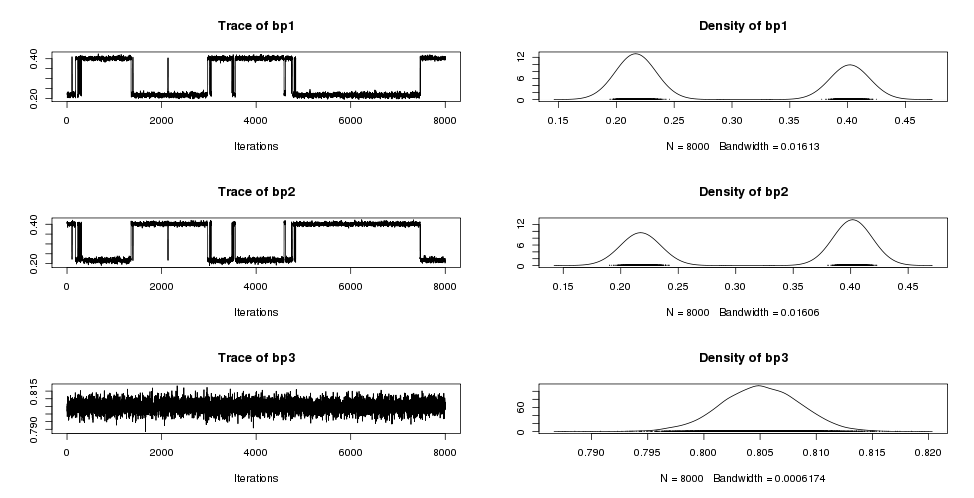
\includegraphics[scale = 0.42]{images/labelBP.png}
\caption{\emph{Trace plots and corresponding marginal density plots for the $\rho_{k}$ parameters of the Binomial mixture. Label-switching is evident for $\rho_{1}$ and $\rho_{2}$ parameters, resulting in bi-modal marginal densities.}}
\label{labelBP-pic}
\end{center}
\end{figure}

Estimating quantities of interest, \eg posterior mean, from the marginal distributions of $\rho_{1}$ and $\rho_{2}$ parameters, would lead to nonsensical answers. The approach chosen for solving this problem is \citet{Stephens2000} relabelling algorithm, which tries to permute the hidden labels of the MCMC output in such a way that the marginal posterior of each parameter is, as far as possible, unimodal. The \emph{label.switching} package of \citet{Papastamoulis2015} is used for running \emph{Stephens} algorithm. 

The outcome of the algorithm is shown in \emph{Fig. \ref{labelBP-stephens-pic}}. Even though the label switching is not completely vanished, the posterior marginal densities of each parameter became unimodal, hence we can compute quantities of interest.
\begin{figure}[!ht]
\begin{center}
 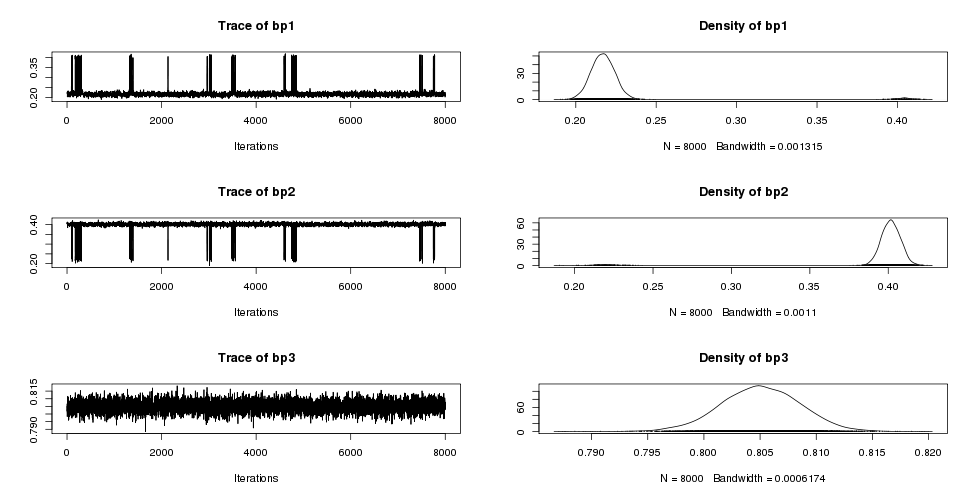
\includegraphics[scale = 0.42]{images/labelBP-stephens.png}
\caption{\emph{Trace plots and corresponding marginal density plots for the $\rho_{k}$ parameters of the Binomial mixture, after running the \citet{Stephens2000} relabelling algorithm. Label switching problem is almost vanished.}}
\label{labelBP-stephens-pic}
\end{center}
\end{figure}
